%%%
%
% $Autor: Wings $
% $Datum: 2021-05-14 $
% $Pfad: GitLab/MLEdgeComputer/General $
% $Dateiname: RaspCamDatasheet
% $Version: 4620 $
%
% !TeX spellcheck = de_DE/GB
%
%%%

\chapter{\TRANS{Datenblätter RaspCAM}{Data Sheets  RaspCAM}}

\section{\TRANS{Datenübersicht}{Data Overview}}

\includegraphics[width=1\textwidth,page=1]{../../MLbib/RaspCam/RaspCamDataSheet.pdf}

\includegraphics[width=1\textwidth,page=2]{../../MLbib/JetsonNano/jetson-nano-module-datasheet-us-1031771-r3-hr.pdf}


\section{\TRANS{Datenblatt Raspberry Pi High Quality Camera}{Data Sheet Raspberry Pi High Quality Camera}}

\newcounter{mycounterRaspCam}
\setcounter{mycounterRaspCam}{1}

\whiledo {\value{mycounterRaspCam} < 7}
{
\includegraphics[width=1\textwidth,page=\themycounterRaspCam]{../../MLbib/RaspCam/RaspCamDataSheet.pdf}
\stepcounter{mycounterRaspCam}
\newpage
}

\section{\TRANS{Datenblatt Raspberry Pi High Quality Camera - Getting started}{Data sheet  Raspberry Pi High Quality Camera - Getting started}}

\setcounter{mycounterRaspCam}{1}

\whiledo {\value{mycounterRaspCam} < 8}
{
    \includegraphics[width=1\textwidth,page=\themycounterRaspCam]{../../MLbib/RaspCam/RaspCamGettingStarted.pdf}
    \stepcounter{mycounterRaspCam}
    \newpage
}

\section{\TRANS{Datenblatt Raspberry Pi High Quality Camera - Bauteilzeichnung}{Data sheet Raspberry Pi High Quality Camera - component drawing}}

\includegraphics[width=1\textwidth,page=1]{../../MLbib/RaspCam/RaspCamDrawing.pdf}
 
\section{\TRANS{Datenblatt Raspberry Pi High Quality Camera - Parameter 6 mm Linse}{Data sheet Raspberry Pi High Quality Camera - Parameter 6 mm lens}}

\includegraphics[width=1\textwidth,page=1]{../../MLbib/RaspCam/RpizCam6mmDataSheet.pdf}

\section{\TRANS{Datenblatt Raspberry Pi High Quality Camera - Montage der Linsen}{Data sheet Raspberry Pi High Quality Camera - Mounting the lenses}}

\includegraphics[height=1\textheight,page=1]{../../MLbib/RaspCam/RpizCam16mmMounting.pdf}

\includegraphics[height=1\textheight,page=1]{../../MLbib/RaspCam/RpizCam6mmMounting.pdf}
